\documentclass{beamer}
\usepackage[utf8x]{inputenc}
\usepackage[ngerman]{babel}
\usepackage{color}
\usepackage{listings}
\usepackage{graphicx} % needed for beamer
\usepackage{cclicenses}

\lstset{%
  language=sh, % FIXME: nice syntax coloring for JSON
  basicstyle=\ttfamily\footnotesize,
	showspaces=false,
	showstringspaces=false,
	showtabs=false,
	keepspaces=true,
	%breaklines=true,
}

\usetheme{Boadilla}
\usefonttheme{professionalfonts}
\useoutertheme[subsection=false,footline=empty]{miniframes}
\useinnertheme{circles}
\setbeamertemplate{footline}[frame number]

\author{Stratum~0~e.~V.}
\title{Cryptoparty}
\subtitle{Sichere Kommunikation im Internet}
\date{17. August 2013}

\begin{document}
\begin{frame}
	\maketitle
\end{frame}

\section{Begrüßung}
\begin{frame}{Begrüßung}
\begin{itemize}
	\item Wer sind wir?
	\item Wer seid ihr?
\end{itemize}
\end{frame}


\section{Organisatorisches}
\begin{frame}{Organisatorisches}
\begin{itemize}
	\item Ablauf:
		\begin{itemize}
			\item kurzer Vortrag zur Theorie (15-20 Min)
			\item Workshop in Kleingruppen
		\end{itemize}
	\item Getränke hinten an der Theke
	\item WLAN-Passwort ist: FIXME
	\item Folien gibts auf \url{https://stratum0.org/cryptoparty}
\end{itemize}
\end{frame}

\section{Einführung}
\begin{frame}{Motivation}
\begin{itemize}
	\item Daten im Internet sind vergleichbar mit Postkarten: \\
		\vfill
		\begin{center}
			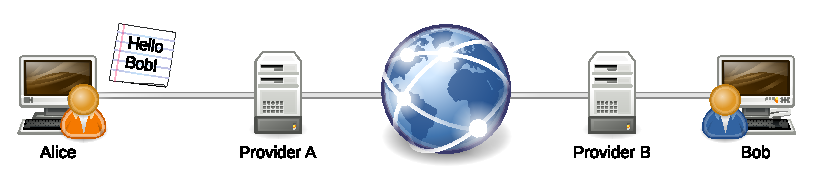
\includegraphics[width=0.8\textwidth]{no-crypto.pdf}
		\end{center}
	\pause
	\vfill
	\item Mögliche Angriffspunkte:
		\begin{itemize}
			\item Provider A
			\item die große Internet-Wolke
			\item Provider B
		\end{itemize}
	\pause
	\vfill
	\item Aber: es gibt Möglichkeiten, das zu verhindern.
\end{itemize}
\end{frame}

\begin{frame}
\begin{block}{Disclaimer}
	\begin{itemize}
		\item Es gibt keine 100-prozentige Sicherheit.
		\item Alles hier gezeigte ist Stand der Technik und hinreichend sicher.
	\end{itemize}

	Trotzdem: plant keine Terroranschläge über das Internet.
\end{block}
\end{frame}

\section{Public-Key-Kryptographie}
\begin{frame}{Public-Key-Kryptografie}
\emph{(Kryptografie: die Lehre vom Geheimen)}

\begin{itemize}
	\item 1977 erfunden von Ron Rivest, Adi Shamir und Leonard Adleman
	\item komplizierte mathematische Verfahren
	\begin{itemize}
		\item soll hier nicht erklärt werden
	\end{itemize}
	\item Jeder Kommunikationsteilnehmer generiert ein zufälliges Schlüsselpaar:
	\begin{itemize}
		\item einen öffentlichen Schlüssel zum Verschlüsseln von Nachrichten
		\item einen geheimen Schlüssel zum Entschlüsseln von Nachrichten
	\end{itemize}
\end{itemize}
\begin{alertblock}{Achtung}
	Der private Schlüssel sollte geheim gehalten werden, der öffentliche Schlüssel
	sollte veröffentlicht werden.
\end{alertblock}
\end{frame}

\begin{frame}{Public-Key-Kryptografie}
	\begin{itemize}
		\item Nachrichten, die mit dem öffentlichen Schlüssel verschlüsselt wurden,
			können nur mit dem passenden privaten Schlüssel entschlüsselt werden
		\vfill
		\begin{center}
			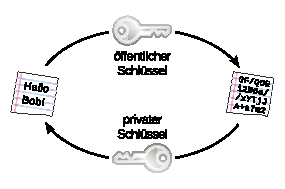
\includegraphics[width=0.5\textwidth]{public-private-keys.pdf}
		\end{center}
		\vfill
		\item der private Schlüssel kann nicht aus dem öffentlichen Schlüssel
			hergeleitet werden
	\end{itemize}
\end{frame}

\begin{frame}{Analogie}
\begin{itemize}
	\item Das ist Bob: \raisebox{-6pt}{
\includegraphics[height=20pt]{bob.pdf}}
	\vspace{0.5\baselineskip}

	\item Bob verteilt Bügelschlösser für jeden, der Nachrichten an ihn
		verschlüsseln will:
		\raisebox{-4pt}{
\includegraphics[height=16pt]{bobs-lock.pdf}}
	\begin{itemize}
		\item öffentlicher Schlüssel
	\end{itemize}
	\vspace{0.5\baselineskip}

	\item Bob behält den Schlüssel für die Schlösser:
		\raisebox{-2pt}{
\includegraphics[width=20pt]{bobs-key.pdf}}
	\begin{itemize}
		\item privater Schlüssel
	\end{itemize}
\end{itemize}
\end{frame}

\begin{frame}{Verschlüsseln und Entschlüsseln}
Alice verschlüsselt eine Nachricht an Bob mit seinem öffentlichen Schlüssel: \\
\begin{center}
	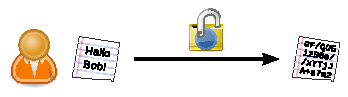
\includegraphics[width=.7\textwidth]{public-key-encryption.pdf}
\end{center}

Nur Bob kann diese Nachricht jetzt mit seinem privaten Schlüssel lesen:
\begin{center}
	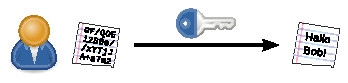
\includegraphics[width=.7\textwidth]{public-key-decryption.pdf}
\end{center}
\end{frame}

\begin{frame}{Signaturen}
Das System auch umgekehrt für Signaturen einsetzbar:
\begin{center}
	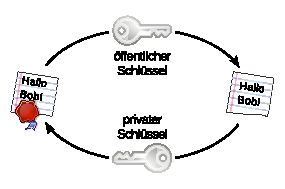
\includegraphics[width=0.5\textwidth]{public-private-signature.pdf}
\end{center}
\begin{itemize}
	\item Bob verschlüsselt ein Dokument mit seinem \emph{privaten} Schlüssel
		\begin{itemize}
			\item nur Bob hat diesen privaten Schlüssel, also kann nur Bob diesen
				Schlüsseltext erstellt haben
		\end{itemize}
	\item Jeder andere kann den Schlüsseltext entschlüsseln und Bobs Signatur
		überprüfen
\end{itemize}
\end{frame}

\begin{frame}{Vertrauensnetzwerke}
\begin{block}{Soweit in Ordnung\ldots}
	Aber wie kann ich sicher sein, dass der Schlüssel, mit dem ich
	Nachrichten verschlüssele, auch wirklich Bob gehört?
\end{block}

\pause
\textbf{Lösung:} Vertrauensnetzwerke
\begin{itemize}
	\item Ich prüfe, ob Alices öffentlicher Schlüssel auch wirklich Alice gehört
	\begin{itemize}
		\item Falls ja, signiere ich ihren öffentlichen Schlüssel
		\item Ich versichere damit, dass Alice diesen Schlüssel besitzt
	\end{itemize}
	\item Alice hat das gleiche mit Bobs Schlüssel getan
	\item Falls Alice nicht schlampig war, kann ich Bobs Schlüssel indirekt
		vertrauen
\end{itemize}
\end{frame}

\begin{frame}{Vertrauensnetzwerke}
Beispiel Vertrauensnetzwerk:
\begin{center}
	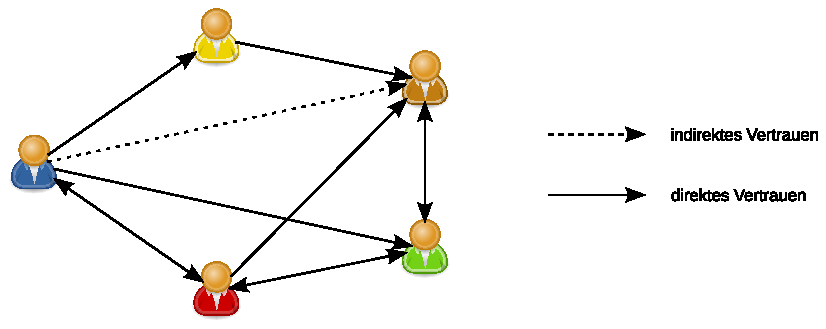
\includegraphics[width=\textwidth]{web-of-trust.pdf}
\end{center}
\end{frame}

\section{Surfen}
\begin{frame}{Sicher surfen: HTTPS}
\begin{itemize}
	\item Webserver besitzt privaten und öffentlichen Schlüssel ("`Zertifikat"')
	\item Schlüsselerzeugung auf Benutzerseite dynamisch
	\item Vertrauensnetzwerk über \emph{Certificate Authorities} (CA)
	\begin{itemize}
		\item nehmen meist Geld für die Signatur des Server-Zertifikats
		\item Identitätsprüfung je nach CA unterschiedlich genau\ldots
		\item Browser vertrauen nur bestimmten CAs $\Rightarrow$
			Zertifikatswarnungen
	\end{itemize}
\end{itemize}
\begin{center}
	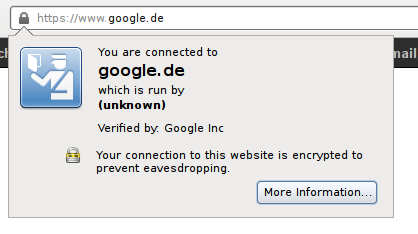
\includegraphics[width=0.5\textwidth]{https-google-de.png}
\end{center}
\end{frame}

\begin{frame}{Sicher surfen: HTTPS}
	\begin{alertblock}{Achtung}
		Die Daten sind nur auf dem Weg zum Webserver geschützt, am Ende liegen sie
		wieder entschlüsselt vor!
	\end{alertblock}

	\begin{itemize}
		\item Auf dem Webserver könnte z.\,B. auch ein Angreifer seine Finger im
			Spiel haben\ldots
		\item Certificate Authorities könnten gefälschte Zertifikate ausstellen
		\begin{itemize}
			\item Beispiel: Comodo CA, DigiNotar, TürkTrust
		\end{itemize}
		\item keine eingebaute Anonymisierung
	\end{itemize}
\end{frame}

\section{E-Mail}
\begin{frame}{Mails verschlüsseln: PGP}
\begin{itemize}
	\item PGP: Pretty Good Privacy ("`Ziemlich gute Privatsphäre"')
	\item seit 1998 ein Standard für Mailverschlüsselung
	\begin{itemize}
		\item Freie Softwarelösung: GnuPG (GNU Privacy Guard)
	\end{itemize}
	\item Verschlüsselt keine Metadaten (wie z.\,B. Betreffzeile)!
	\item Erweiterungen für viele Mailprogramme vorhanden
\begin{alertblock}{Webbasierte Dienste?}
	Mit webbasierte Diensten ist PGP kaum möglich -- es ist nötig, ein
	Mailprogramm auf dem eigenen Rechner zu installieren! Die meisten Anbieter
	bieten Anleitungen zum Einrichten der Mailkonten im Mailprogramm an.
\end{alertblock}
\end{itemize}
\end{frame}

\begin{frame}{PGP: Softwareunterstützung}
\begin{itemize}
	\item Windows: Gpg4Win, \url{http://gpg4win.org/}
	\item Mac OS X: GPGTools, \url{https://www.gpgtools.org/}
	\item Linux: GnuPG, \url{http://gnupg.org}
\end{itemize}

Darauf aufbauend Unterstützung in Mailprogrammen:
\begin{itemize}
	\item Mozilla Thunderbird: Enigmail, \url{http://enigmail.org}
	\item Apple Mail: GPGMail, \url{https://www.gpgtools.org/}
	\item Microsoft Outlook: Gpg4Win
\end{itemize}
\end{frame}

\section{Chats}
\begin{frame}{Chats verschlüsseln: OTR}
\begin{itemize}
	\item OTR: Off-the-Record Messaging
	\item Verschlüsselung
	\item Authentizität
	\item Abstreitbarkeit
		\begin{itemize}
			\item keiner kann nachher beweisen, ich hätte etwas bestimmtes gesendet
		\end{itemize}
	\item Folgenlosigkeit
		\begin{itemize}
			\item Verlust des privaten Schlüssels hat keine Auswirkung auf bisherige
				Verbindungen
		\end{itemize}
\end{itemize}
\end{frame}

\begin{frame}{OTR: Softwareunterstützung}
\begin{itemize}
	\item eingebaut in Adium (Mac OS X), Jitsi, Xabber (Android), ChatSecure (iOS)
	\item Pidgin (Windows, Linux): \url{http://www.cypherpunks.ca/otr/}
	\item Miranda (Windows): auf der Addons-Seite
\end{itemize}

\begin{block}{Tipp}
	Adium, Pidgin und Miranda unterstützen alle gängigen Netzwerke, z.~B. ICQ,
	MSN, Yahoo und auch Facebook Chat.
\end{block}
\end{frame}

\begin{frame}{Weitere Informationen}
\begin{itemize}
	\item CryptoCD, Anleitungen auf deutsch, 
		\url{http://www.cryptocd.org/CryptoCDBetriebssystem}
	\item Cryptoparty Handbook, mit Anleitungen zu allen hier gezeigten Themen
		(englisch), \url{https://www.cryptoparty.in/documentation/handbook}
\end{itemize}
\end{frame}

\begin{frame}{Lizenz}
\begin{center}
Dieses Dokument steht unter der Lizenz CC-BY-SA 3.0 Unported, siehe
\url{https://creativecommons.org/licenses/by-sa/3.0/deed}.

\cc\bysa
\end{center}

\footnotesize
Folgende Symbole wurden benutzt:
\begin{itemize}
	\item Server-Symbol, Computer-Symbol: Tangerine Icon Theme, CC-BY-SA 2.5,
		Copyright 2004-2006 Canonical Ltd.
		\url{https://launchpad.net/tangerine-icon-theme}
	\item Schlüssel-Symbol: aus dem Gnome Icon Theme, CC-BY-SA 3.0 United States,
		Copyright GNOME Project
	\item Notizblock-Symbol:
		\url{http://commons.wikimedia.org/wiki/File:Ruled_paper_note_with_pin.svg},
		Autor: Andreas Plank, CC-BY-SA-3.0 Unported
	\item alle anderen Symbole: Tango Desktop Project, gemeinfrei.
		\url{http://tango.freedesktop.org}
\end{itemize}
\end{frame}

\end{document}
